% gc-lab-10-optimization.tex

\documentclass[11pt]{article}
\usepackage{enumerate}
\usepackage{syllogism} 
\usepackage{october}
\usepackage[table]{xcolor}

\newcounter{aufg}
\setcounter{aufg}{0}
\newcommand{\aufgabe}[0]{\refstepcounter{aufg}\textbf{(\arabic{aufg})}}

\begin{document}

\textbf{Optimization}

\emph{\CourseName, \CourseNumber}

% solutions are in cooleyopt.html

{\aufgabe} The cost of fuel for running a train is proportional to the
square of the speed maintained, and is \$50 per hour when the speed is
20 mph. Other charges, such as labour, for example, are \$200 per
hour. What should be the speed for a 500-mile trip in order that the
total cost shall be as little as possible?

{\aufgabe} The product of the concentration of hydrogen ions,
$C_{h^{+}}$, and hydroxyl ions, $C_{oh^{-}}$, in any aqueous solution
is a constant $=10^{-14}$. At what concentration of hydrogen ions will
the sum of hydrogen ions and hydroxyl ions be a minimum?

{\aufgabe} Find the number that exceeds its square by the greatest
amount.

{\aufgabe} A rectangular garden is to be surrounded by a fence and
divided into two equal parts by a fence parallel to one side. If the
area is to be 600 square feet, what should be the dimensions in order
to require the least amount of fencing?

{\aufgabe} Find the dimensions (height and radius) of the largest (in
volume) right circular cylinder that can be inscribed in a sphere six
inches in diameter.

\begin{figure}[h]
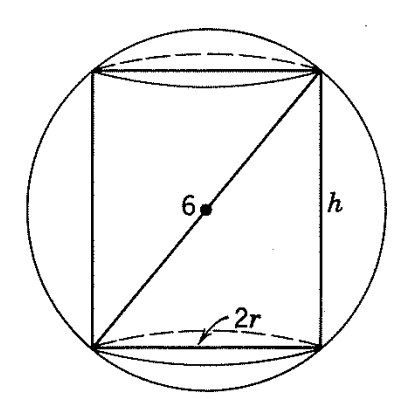
\includegraphics[scale=.4]{./diagrams/cooleyopt.png}
\end{figure}

\end{document}

